%%%%%%%%%%%%%%%%%%%%%%%%%%%%%%%%%%%%%%%%%%%%%%%%%%%%%%%%%%%%%%%%%%
%%%%%%%% ICML 2014 EXAMPLE LATEX SUBMISSION FILE %%%%%%%%%%%%%%%%%
%%%%%%%%%%%%%%%%%%%%%%%%%%%%%%%%%%%%%%%%%%%%%%%%%%%%%%%%%%%%%%%%%%
\documentclass{article}
\usepackage{times}
\usepackage{graphicx} % more modern
\usepackage{subfigure} 
% For citations
\usepackage{natbib}
% For algorithms
\usepackage{algorithm}
\usepackage{algorithmic}

% Stuff that I added in (Daniel Seita) 
\usepackage{amsmath,amssymb,amsthm,verbatim}
\graphicspath{ {Images/} }

% As of 2011, we use the hyperref package to produce hyperlinks in the
% resulting PDF.  If this breaks your system, please commend out the
% following usepackage line and replace \usepackage{icml2014} with
% \usepackage[nohyperref]{icml2014} above.
\usepackage{hyperref}

% Packages hyperref and algorithmic misbehave sometimes.  We can fix
% this with the following command.
\newcommand{\theHalgorithm}{\arabic{algorithm}}

% Employ the following version of the ``usepackage'' statement for
% submitting the draft version of the paper for review.  This will set
% the note in the first column to ``Under review.  Do not distribute.''
%\usepackage{icml2014} 
% Employ this version of the ``usepackage'' statement after the paper has
% been accepted, when creating the final version.  This will set the
% note in the first column to ``Proceedings of the...''
\usepackage[accepted]{icml2014}

% The \icmltitle you define below is probably too long as a header.
% Therefore, a short form for the running title is supplied here:
\icmltitlerunning{The Distributed Retired Traveling Salesman Problem}

\begin{document} 

\twocolumn[
\icmltitle{The Distributed Retired Traveling Salesman Problem}

% It is OKAY to include author information, even for blind
% submissions: the style file will automatically remove it for you
% unless you've provided the [accepted] option to the icml2014
% package.
\icmlauthor{Daniel Seita}{dts1@williams.edu}
\icmlauthor{Ziang Zhang}{zz2@williams.edu}
\icmladdress{Department of Computer Science, Williams College, Williamstown, MA 01267 USA}

% You may provide any keywords that you 
% find helpful for describing your paper; these are used to populate 
% the "keywords" metadata in the PDF but will not be shown in the document
\icmlkeywords{distributed systems}

\vskip 0.3in
]

\begin{abstract} 
The use of major online travel agencies has made scheduling long-term travel much easier by allowing users to easily select a set of flights to
purchase tickets from. Current travel agencies allow users to plan out trips involving airlines to more than one major city, but they require (1)
specific dates for each city and (2) an ordering. We propose a system that does not require to burden the user with this type of decision.  It
essentially solves a harder version of the Traveling Salesman Problem since costs are not constant between two cities.  Assuming the number of cities
is limited to a reasonable number for a trip (e.g., four) then this algorithm should successfully find the cheapest cost flight under a number of weak
assumptions. We present the theoretical and systematic components of the project, discuss empirical results, and suggest future work.
\end{abstract} 

\section{Introduction and Motivation}\label{sec:intro}

The use of major online travel agencies, such as Travelocity and Kayak, has made scheduling long-term travel much easier by allowing users to easily
select a set of flights to purchase tickets from. People use a combination of factors to help them make their decision, such as the price of all the
flights and the days they wish to land and depart from a city. Current travel agencies allow users to plan out trips involving airlines to more than
one major city, but they require (1) specific dates for each city and (2) an ordering.

For instance, if the first author of this paper wants to visit Paris, London, and Tokyo from June 1 to July 1, and he starts out in New York City
(NYC), he may want to schedule flights such that he departs from NYC to arrive in Paris on June 1, and then departs from Paris so that he arrives in
London on June 10, and then depart there to be in Tokyo on June 20, and then fly back to NYC on July 1. But suppose the first author is retired (and
presumably, is rich, or stole money from the second author). Thus, he has substantial free time, so he is not restricted on which days he can be in
particular cities. He is still prudent, so he wants to schedule trips such that airline travel costs are \emph{minimal}. This is challenging using
current agencies, which motivates us to produce a more general service that can solve this problem:

\begin{itemize}
    \item a date range from $X$ to $Y$ (with $X$ occurring earlier than $Y$),
    \item and a list of destinations to reach, $d_1, d_2, \ldots, d_m$, with $d_1$ equal to $d_m$ only if the user wants to end up at the same spot
where he started. (We assume for the sake of realism that these destinations are all reachable by air travel; a number of other assumptions will be
discussed in Section~\ref{sec:limitations})
\end{itemize}

The goal is to find the \textbf{cheapest}, valid schedule of flights $f_1, f_2, \ldots, f_n$, with $n > m$, such that it touches each city at least
once\footnote{The cheapest route of flights to visit these cities may, in fact, require the traveler to visit an airport more than once.}. We will use
the Matrix Airfare Search\footnote{\url{http://matrix.itasoftware.com/}} database to obtain information about our flights; the information itself will
be extracted with our own web crawler. We coin this ``The Retired Traveler Problem,'' primarily because if we assume the dates are set far enough
apart, it would interfere with a non-retired person's occupation. For details on the real problem, see sources such as~\cite{Applegate:2007:TSP:1374811}.

Our project is a combination of mathematics and systems. Sections~\ref{sec:math} and~\ref{sec:systems} describe our objectives in further detail.

\section{Mathematical Component}\label{sec:math}

\subsection{An Integer Programming Formulation}

We will solve this problem using a technique known as \textbf{integer programming}. This is loosely based off of the many ways of solving the
\emph{traveling salesman problem}, where the goal is to hit each city exactly once with fixed costs. Our problem is more difficult than the traveling
salesman problem, because our costs are not fixed. The cheapest way of going from city $i$ to city $j$ will vary depending on the day. (The other
major difference between our problem and the traveling salesman problem is that we are assuming we can touch each city more than once\footnote{This
may not actually make our problem much harder but the varying costs certainly will.}.)

We define our problem formulation as follows.

\begin{itemize}
    \item We have $n$ cities to reach; we index cities by $i$ or $j$ (where $i, j \in \{1, 2, \ldots, n\}$).
    \item We have $t$ (consecutive) days when we can travel: $t \in \{1, 2, \ldots, m\}$. Let
    \item The minimum cost for traveling from city $i$ to $j$ on day $t$ is $c_{ijt}$. To start out this project, we assume that all flights span one
day and are not overnight, for simplicity. As soon as possible, we will expand this to include potential hub stops, overnight flights, etc.
\end{itemize}

This allows us to define the following binary variables:

\[
x_{ijt} = \begin{cases}
1 &\mbox{if we go from cities } i \mbox{ to } j \mbox{ on day } t, \\ 
0 & \mbox{otherwise}.
\end{cases}
\]

The goal is to solve this problem:

\begin{equation}
\mbox{Minimize } \sum_{t=1}^{m} \sum_{i=1}^{n} \sum_{j=1}^{n} c_{ijt}x_{ijt},
\end{equation}

\textbf{subject to} the following constraints:

\begin{align}
\sum_{i=1}^{n} \sum_{j=1}^{n} x_{ijt} &\le 1 \mbox{ for all } t \in \{1, 2, \ldots, m\}, \\ 
\sum_{t=1}^{m} \sum_{i=1}^{n} x_{ijt} &\ge 1 \mbox{ for all } j \in \{1, 2, \ldots, n\}, \\
\sum_{t=1}^{m} \sum_{j=1}^{n} x_{ijt} &\ge 1 \mbox{ for all } i \in \{1, 2, \ldots, n\}.
\end{align}

The first constraint ensures that we have at most one flight per day. The second constraint ensures we enter each city at least once. The third
constraint ensures we leave each city at least once. Sadly, this is \textbf{not} enough to solve our problem! The issue here is with potential cycles.
Figure~\ref{fig:bad_solution} shows how the integer programming solution could theoretically give us a solution consisting of disjoint cycles.

\begin{figure}[t]
\vskip 0.2in
\begin{center}
\centerline{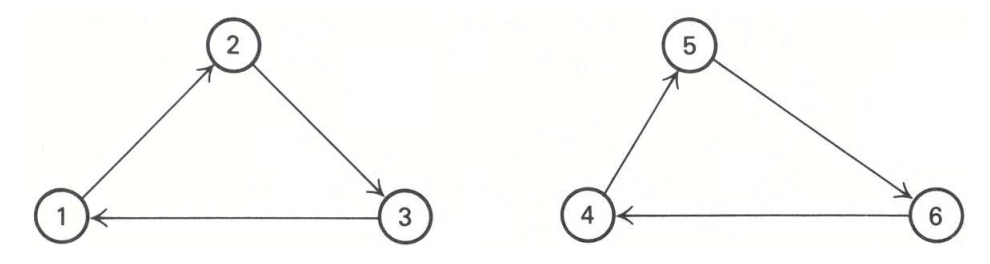
\includegraphics[width=\columnwidth]{bad_solution}}
\caption{This represents two sets of disjoint cycles.}
\label{fig:bad_solution}
\end{center}
\vskip -0.2in
\end{figure}

To counteract this issue, we will need to ensure we have additional variables. With the six-variable situation in Figure~\ref{fig:bad_solution}, for
instance, we will need constraints such as

\begin{equation}
\sum_{t=1}^{m} (x_{14t} + x_{15t} + x_{16t} + x_{24t} + x_{25t} + x_{26t} + x_{34t} + x_{35t} + x_{36t}) \ge 1.
\end{equation}

The previous constraint ensures that at least one leg of the tour connects cities 1, 2, and 3 with cities 4, 5, and 6. We need constraints like these
for every way we can split up the cities into groups. Of course, the need to implement these kind of constraints to prevent sub-tours is why integer
programming is so difficult. Fortunately, we will assume the user is going to keep the number of cities reasonably small.

\subsection{Implementation Details}

How to best implement this is still an open question. There are algorithms for implementing integer programming. The question is whether we
can efficiently use our \emph{distributed systems}. There are a number of results based on parallelizing integer programming in the literature. We
will read through them and by the first checkpoint (see Section~\ref{sec:checkpoint1}) we will have made a decision. There are also some online
implementations, such as CPLEX Optimizer\footnote{\url{http://www-01.ibm.com/software/commerce/optimization/cplex-optimizer/index.html}}, but I think
it is in our best interests to implement this ourselves.

\section{Systems Component}\label{sec:systems}

\begin{figure}[t]
\vskip 0.2in
\begin{center}
\centerline{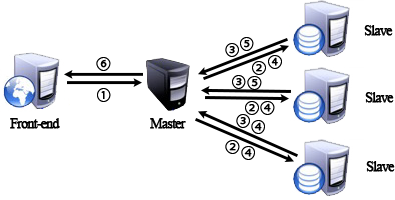
\includegraphics[width=\columnwidth]{servers}}
\caption{This represents our ideal machine setup.}
\label{fig:machines}
\end{center}
\vskip -0.2in
\end{figure}

We will have a front-end server, a master server, and a group of slave servers in the system, as shown in Figure~\ref{fig:machines}. We get all the
servers from the PlanetLab Platform (thanks to Jeannie).

\subsection{Front-end Server}
This server will serve as a front-end interface for the ignorant masses. It receives user input, forwards the request to the master server (shown in
the image as step \texttt{1}), listens to the master for the result (shown as step \texttt{6}), and displays the result when it is ready. More
specifically, the front-end server will have a simple website to interact with the user.

\subsection{Master Server}
The Master server is the brain of the system. It listens to the user request sent from the front-end server (step \texttt{1}). When a request comes
in, it first comes up with a list of flight prices on all possible dates and for all possible destinations in the problem that we need to get for the
computation, distributes the flight price queries among all the slaves (step \texttt{2}), gathers all the price data back from the slaves (step
\texttt{3}), and combines them. It then upload the combined data to a distributed file system to make the data available for parallel computing on all
the slaves. Then it starts the parallel computing for the cheapest route using a distributed zero-one linear programming algorithm on all slaves
(steps \texttt{4} and \texttt{5}). After the computation, it sends the results of the cheapest route back to the front-end server (step \texttt{6}).

\subsection{Slave Server}
We have a group of slave servers that listens to the command of the master server and does the distributed tasks of flight price querying (using the
web crawler we write) and parallel zero-one linear programming.

\section{Checkpoints}

\subsection{Checkpoint 5/2}\label{sec:checkpoint1}

By this date, we will have our machine/cluster and the web crawler working. We will finalize the mathematical portion of our work by choosing which
distributed algorithm to implement.

\subsection{Checkpoint 5/9}\label{sec:checkpoint2}

By this date, we will have implemented (1) the distributed systems requesting process\footnote{As stated earlier, this is when the master distributes
requests to slave machines to determine the cheapest flight for a certain date and city destinations.} and (2) the (possibly distributed) integer
programming problem.  In other words, the code will solve the problem for the two of us any reasonable input (it just lacks a front-end for the rest
of the ignorant masses). \\

{\bf UPDATE!!!} \\

We are now at the second checkpoint. Here is what we have accomplished:

\begin{itemize}
    \item We have implemented a web crawler
    \item We have implemented a web crawler server that can talk to the crawler to get the price
    \item We have implemented Balas' Additive Algorithm~\cite{doi:10.1287/opre.13.4.517} for efficiently solving binary integer programming problems.
    \item We have gotten the basic setup for our writeup (i.e., this PDF document) ... it just needs to be heavily revised.
\end{itemize}

We have sent all of our code to Jeannie by email.

I (Daniel Seita) have to admit that we're a bit behind where we want, because we haven't been able to actually combine our crawler's results with the
input to the integer programming problem, but we're going to do nothing but 339 work over the weekend. We're also thinking of expanding the work to
include other integer programming formulations (this is going to be an additional part of our mathematical side of this project).

\subsection{Presentation and Final Product}

By this date, we will have implemented a fancy front-end website where users can query a flight schedule. We will also be prepared to give a talk by
the May 13 ({\bf UPDATE: May 11}) date. Then we will work on fixing up this paper and doing some more programming.

\section{Limtiations}\label{sec:limitations}

{\bf TODO}

\section{Conclusions and Future Work}\label{sec:conclusions}

{\bf TODO}

\section*{Acknowledgments}
 
{\bf TODO}

\bibliography{Daniel_Lucky_Report}
\bibliographystyle{icml2014}

\end{document} 

% Look at that! Andrea is here! ~Daniel Seita (05/08/2014)

% This document was modified from the file originally made available by
% Pat Langley and Andrea Danyluk for ICML-2K. This version was
% created by Lise Getoor and Tobias Scheffer, it was slightly modified  
% from the 2010 version by Thorsten Joachims & Johannes Fuernkranz, 
% slightly modified from the 2009 version by Kiri Wagstaff and 
% Sam Roweis's 2008 version, which is slightly modified from 
% Prasad Tadepalli's 2007 version which is a lightly 
% changed version of the previous year's version by Andrew Moore, 
% which was in turn edited from those of Kristian Kersting and 
% Codrina Lauth. Alex Smola contributed to the algorithmic style files.  
